\documentclass[runningheads]{llncs}

\usepackage[T1]{fontenc}
\usepackage{amsmath}
\usepackage{amssymb}
\usepackage{booktabs}
\usepackage{float}
\usepackage{graphicx}
\usepackage[hidelinks]{hyperref}
\usepackage{url}

\begin{document}

\title{Auditing Counterfactual Data Augmentation in Reinforcement Learning}
\titlerunning{Auditing Counterfactual Data Augmentation}

\author{Sajan Kumar \and Shilpa Noushad \and Pratyush Uppuluri}
\authorrunning{S. Kumar et al.}
\institute{Purdue University, West Lafayette, IN, USA}

\maketitle

\begin{abstract}
We audit a ground-up reimplementation of CTRL, which augments offline
reinforcement-learning data by inferring and reusing transition-specific
exogenous noise. The audit separates three questions that an end-to-end score
conflates: whether the environment is learnable, whether exact noise reuse helps,
and whether a learned structural causal model can approximate the corresponding
counterfactuals. A reported-architecture D3QN attempt does not recover the CartPole
performance plotted by Lu et al. A disclosed stabilized learner does recover the
same numerical range, but is not a faithful reproduction. We then run a frozen,
paired 30-seed mechanism study using exact simulator transitions. After matching
synthetic-pool size, optimizer updates, and within-transition noise sharing,
oracle reuse of factual noise scores 62.78 return points below an independently
drawn shared-noise control on clean evaluation (95\% paired bootstrap interval
$[-111.31,-14.56]$). Under our process-noise stress test, the difference is
$-2.05$ and meets a study-defined $\pm5$ practical-equivalence rule. Finally, a
positive-weight BiCoGAN candidate fails held-out transition, termination, and
latent-calibration gates in all five development seeds. Thus, instance-specific
noise reuse is not sufficient to outperform the matched fresh-shared control in
this setting, and the
present implementation does not validate learned counterfactual augmentation.
\keywords{causal reinforcement learning \and counterfactual augmentation \and
offline reinforcement learning \and reproducibility}
\end{abstract}

\section{Introduction}

Counterfactual augmentation promises to improve data efficiency without further
environment interaction. In a structural causal model (SCM), dynamics are
represented as
\begin{equation}
S_{t+1}=f(S_t,A_t,U_{t+1}),
\label{eq:scm}
\end{equation}
where $U_{t+1}$ contains exogenous factors. For an observed transition, a
counterfactual first abducts its realized $u_{t+1}$ and then changes the action
while holding that realization fixed. This differs from sampling new noise,
which produces another transition-distribution draw rather than an individual
counterfactual~\cite{pearl2009causality,buesing2019cfgps}.

CTRL applies this idea to offline reinforcement learning (RL): a Bidirectional
Conditional Generative Adversarial Network (BiCoGAN) estimates the forward
mechanism and inverse noise mapping, after which a Dueling Double Deep
Q-Network (D3QN) is trained on real and generated
transitions~\cite{lu2020ctrl,jaiswal2019bicogan}. Lu et al. report
strong CartPole sample efficiency, but provide no official implementation and
leave consequential details unspecified, including failure handling, generated
data mixing, convergence criteria, and whether state noise is process or sensor
noise. Our original manuscript treated exploratory, incompatible experiments as
evidence for a broad conditional benefit. This revision withdraws those claims
and asks a narrower, auditable question: \emph{what does transition-specific
noise reuse add when the simulator mechanism is known exactly?}

Our contributions are:
\begin{itemize}
  \item a direct, protocol-qualified comparison with Lu et al., plus learner,
  environment, and protocol diagnostics that expose a failed reproduction;
  \item two separate paired 30-seed simulator studies, including a follow-up that matches
  noise sharing and isolates factual coupling from synthetic-pool diversity; and
  \item a held-out model-quality gate showing why the attempted learned BiCoGAN
  cannot support a downstream learned-counterfactual claim.
\end{itemize}

\section{Background and Related Work}

Lu et al. prove counterfactual identifiability when $f(s,a,\cdot)$ is strictly
monotone and give Q-learning convergence results under their stated
assumptions~\cite{lu2020ctrl}. Standard neural networks do not provide this
property automatically. Positive-weight and constrained monotonic networks are
possible implementation directions~\cite{runje2023monotonic}, while recent work
clarifies that counterfactual identification depends on recoverability of the
exogenous structure~\cite{chen2025exogenous}.

The literature after CTRL also makes clear that augmentation quality and scope
must be controlled. CoDA and MoCoDA exploit locally factored dynamics
~\cite{pitis2020coda,pitis2022mocoda}; ACAMDA uses guided adversarial
counterfactual estimation~\cite{sun2024acamda}; and CAIAC limits augmentation
using causal action influence~\cite{armengolurpi2024caiac}. Causal state and
transfer representations address related generalization questions
~\cite{huang2022asr,huang2022adarl}; Deng et al. provide a broader causal-RL
survey~\cite{deng2023survey}. Our study does not compete with these methods. It
is a diagnostic of the simpler CTRL mechanism and the evidence required before
a learned augmentation result is reported.

\section{Audit Design}

\subsection{CartPole-SD protocol}

We reconstruct the Simple Dataset (SD) setting described by Lu et al.: 250
random-action trials, at most 20 consecutive transitions per trial, 11 actions,
and Gaussian state and action noise with standard deviation 0.05. A commanded
action $a\in\{0,\ldots,10\}$ maps to $a/10$; after action noise $\epsilon_a$,
the applied force is $[2(a/10+\epsilon_a)-1]10$. State noise is added after one
physics step. Our main protocol feeds the noisy next state into subsequent
physics, making it explicit \emph{process noise}. Termination is computed from
the pre-state-noise next state, and collection stops on failure. The resulting
factual datasets in the frozen follow-up contain 3,365--3,705 transitions rather
than exactly 5,000.

\textbf{Clean evaluation} uses the same 11-action simulator with both noise
terms disabled. \textbf{Process-noise evaluation} uses both standard deviations
at 0.05. Both have a 500-step ceiling. We do not call the latter the original
``CTRL/noisy'' protocol because Lu et al. do not specify evaluation noise. Each
policy is evaluated on the same 100 episode seeds. Evaluation episodes are
nested measurements; the training/data seed is the experimental unit.

Table~\ref{tab:protocol-differences} separates reported facts from choices that
cannot be recovered from the original text. These gaps prevent a claim of exact
implementation equivalence even when nominal sample count and architecture are
matched.

\begin{table}[H]
\centering
\caption{Reproduction target and disclosed protocol differences. NR means not
reported by Lu et al.}
\label{tab:protocol-differences}
\small
\begin{tabular}{@{}p{0.24\linewidth}p{0.31\linewidth}p{0.36\linewidth}@{}}
\toprule
Feature & Lu et al. & This audit \\
\midrule
Collection & 250 random-action trials; 20 steps; 11 actions; 0.05 state/action noise
& Same nominal design; failures stop collection in the primary protocol \\
Factual transitions & Figure indexed by sample count; 5,000 shown & 3,365--3,705 in the frozen follow-up; 5,000 tested by continuation diagnostic \\
State-noise semantics & Process versus sensor interpretation NR & Process noise primary; observation-noise sensitivity analysis \\
Evaluation & Ten trials; noise and seed policy NR & 100 fixed episode seeds; clean and process-noise evaluations reported separately \\
Learner budget & Train to convergence & 10,000 updates for architecture check; 5,000 for stabilized mechanism study \\
Generated-data mixing & NR & Fixed 50:50 real/generated minibatches, batch size 256 \\
Downstream learner & Four 512-unit D3QN layers & Same architecture first; then disclosed 2x256 D3QN+CQL stabilization \\
\bottomrule
\end{tabular}
\end{table}

\subsection{Evidence tiers and learners}

Development runs are separated from frozen multi-seed studies. First, we test
the reported four-layer, 512-unit, batch-normalized D3QN architecture
~\cite{wang2016dueling,vanhasselt2016double}. It fails a real-data learner gate.
For the mechanism study only, we select a stabilized learner using real-data
development runs: two 256-unit hidden layers, no batch normalization, Adam with
learning rate $10^{-4}$, Polyak coefficient 0.005, 5,000 updates, and a
Conservative Q-Learning (CQL) coefficient of 0.05~\cite{kumar2020cql}. This
deviation is central: it cannot rescue a faithful reproduction claim.

\subsection{Noise-reuse controls}

For each factual transition and each of its ten alternative actions, the exact
simulator constructs:
\begin{itemize}
  \item \textbf{Fresh-independent synthetic}: draw new action and state noise
  separately for each alternative action;
  \item \textbf{Fresh-shared synthetic}: draw one independent noise pair per
  factual transition and reuse it over all ten alternative actions; and
  \item \textbf{Oracle CF}: reuse the factual transition's action and state
  noise over all ten alternative actions.
\end{itemize}
Fresh-shared and oracle have the same number of noise draws and sibling-sharing
structure; they differ in whether noise is coupled to the factual outcome.
Factual arrays are asserted exactly equal across arms. CartPole reward is fixed
at one per retained transition, and the simulator recomputes the terminal label
for every generated next state. Every learned arm uses the same initialization
and number of updates. Generated arms sample fixed
50:50 real/generated minibatches of size 256, so augmentation does not increase
optimizer steps or minibatch size.

The local follow-up manifest fixes seeds 1030--1059 before execution. Its primary
contrast is oracle minus fresh-shared clean return. Secondary contrasts are the
same comparison under process noise and fresh-shared minus fresh-independent
under both evaluations. The study-defined operational thresholds are 25
clean-return points and 5 process-noise points; they are design choices, not
externally validated standards.

\subsection{Learned-SCM gate}

We also implement a positive-weight BiCoGAN candidate with the layer widths
reported by Lu et al. The generator is coordinatewise nondecreasing in its
four-dimensional latent; this is not claimed to prove strict identifiability.
It is trained on all factual trials and evaluated on an independent 50-trial
bank. Before downstream use, all five development seeds must satisfy: learned-CF
normalized mean-squared error (MSE) at least 20\% below fresh-noise MSE, terminal disagreement below
5\%, every latent standard deviation in $[0.5,2]$, and action reconstruction
MSE at least 10\% below a central-action predictor.

\subsection{Statistical analysis}

We report seed-level mean and standard deviation, median, paired deltas, 95\%
paired bootstrap intervals, paired $t$, Wilcoxon, and sign-randomization tests,
and Holm-adjusted values across the four manifest-specified contrasts. The raw primary
test is reported because that contrast was fixed first; adjusted values are a
familywise sensitivity analysis. A practical-equivalence label requires the
paired 90\% bootstrap interval to lie within its study-defined band. Given
bounded, ceiling-heavy RL returns, paired distributions and sensitivity across
tests are emphasized over a single $p$-value~\cite{agarwal2021precipice}.

\subsection{AI-assisted workflow disclosure}

We used OpenAI Codex with GPT-5.6 Luna (medium reasoning) and GPT-5.6 Sol
(high reasoning), as identified by the run metadata, accessed August
31--September 1, 2026, for experiment-audit
planning, code and test scaffolding, statistical cross-checks, citation
verification, and language editing. The following is a condensed initiating
directive; the supplementary disclosure preserves the verbatim prompt:
\begin{quote}\small
``Can you create create a plan on whatever improvements we can right now. Run
them using subagents using luna model as its cheaper to run through them and use
them whenever low reasoning is required. Then use sol at high effort to analysis
and plan next move until you can't think of anything and we reached at point
where we can edit the latex with comments we got before it gets published.''
\end{quote}
The supplementary disclosure records the focused audit prompts and their roles.
OpenAI Deep Research and Google Deep Research critiques supplied by the authors
were also used to identify literature, protocol, and reporting risks. Their
verbatim initiating prompts and underlying model identifiers were not present
in the supplied records; the supplementary disclosure records this limitation
and gives non-verbatim scope reconstructions. No reported number was taken from
either critique: retained claims, citations, and result artifacts were checked
against primary sources or included raw files.
No generative image model was used; all figures are deterministic plots of the
included result artifacts. The authors inspected the source, raw artifacts,
statistical recomputations, references, and rendered manuscript and retain full
responsibility for the design, claims, citations, and submitted text.

\section{Results}

\subsection{The reported-architecture reproduction fails}

Lu et al. provide CartPole-SD results only in Figure 2(a). Vector-path
inspection, rounded to the nearest ten, gives approximately 260 for D3QN and
310 for CTRLg at 5,000 samples. Their models train to convergence and are tested
for ten trials, but training-seed uncertainty and evaluation noise are not
given. Table~\ref{tab:direct} therefore gives descriptive context only.

\begin{table}[H]
\centering
\caption{Protocol-qualified comparison with Lu et al. Plot values are
approximate; NR means not reported, and no cross-paper statistical comparison
is made.}
\label{tab:direct}
\small
\begin{tabular}{@{}p{0.29\linewidth}ccp{0.34\linewidth}@{}}
\toprule
Setting & Train seeds & Reported return & Protocol/budget note \\
\midrule
Lu D3QN & NR & $\approx260$ & 5,000 samples; eval. noise NR \\
Lu CTRLg & NR & $\approx310$ & BiCoGAN CF; eval. noise NR \\
Our reported-architecture D3QN & 5 & $31.19\pm6.84$ & mean 3,556 transitions; clean eval. \\
Our stabilized real-only ($2\times256$+CQL) & 30 & $266.09\pm162.59$ & 5,000 updates; clean eval. \\
\bottomrule
\end{tabular}
\end{table}

A ten-seed protocol matrix does not repair the reported network: clean
means range from 18.35 to 34.56 across the state-noise and trial-continuation
variants. Continuing every trial to exactly 20 transitions changes
the process-noise clean mean from 32.34 to 34.56. In contrast, a ten-seed online
DQN control, selected on a separate validation seed bank and reported on a
disjoint test bank, reaches $431.00\pm66.12$ clean and $46.88\pm3.21$ under process
noise, versus random $27.15\pm0.96$ and $17.86\pm0.52$. The environment is
learnable; the failure is specific to the attempted offline reproduction.

\subsection{Initial oracle study motivates a matched control}

In an initial paired 30-seed simulator study, oracle CF scored 55.40 points
below fresh-independent synthetic augmentation on clean evaluation (95\% paired
bootstrap interval $[-98.94,-9.54]$). That comparison changed both factual-noise
coupling and the number and dependence of noise draws among ten synthetic
siblings. We therefore treat it as motivating evidence, not the primary
mechanism result, and designed the sibling-sharing-matched follow-up below. The two
cohorts are not pooled.

\subsection{Matched oracle coupling study}

Table~\ref{tab:arms} reports the follow-up's 30 distinct training/data seeds.
The stabilized real-only arm is in the numerical range of Lu et al.'s plot, but
its large dispersion and changed learner preclude a reproduction claim.

\begin{table}[H]
\centering
\caption{Follow-up return across 30 seeds (mean $\pm$ SD; median).}
\label{tab:arms}
\small
\begin{tabular}{@{}lrr@{}}
\toprule
Arm & Clean & Process noise \\
\midrule
Random & $27.03\pm1.52;\ 27.20$ & $17.44\pm0.99;\ 17.60$ \\
Real only & $266.09\pm162.59;\ 224.48$ & $27.51\pm4.81;\ 27.53$ \\
Fresh-independent & $322.27\pm139.54;\ 292.78$ & $37.94\pm2.85;\ 37.98$ \\
Fresh-shared & $367.15\pm140.23;\ 429.66$ & $37.34\pm3.49;\ 38.25$ \\
Oracle CF & $304.37\pm136.75;\ 279.50$ & $35.29\pm3.52;\ 35.58$ \\
\bottomrule
\end{tabular}
\end{table}

Table~\ref{tab:contrasts} reports every manifest-specified contrast rather than
only the primary comparison. The three $p$-values in each cell are from the
paired $t$, Wilcoxon, and sign-randomization tests, respectively.

\begin{table}[H]
\centering
\caption{Paired follow-up contrasts over 30 training seeds. Intervals are 95\%
paired bootstrap intervals; $p$ columns list $t$/Wilcoxon/randomization.}
\label{tab:contrasts}
\scriptsize
\begin{tabular}{@{}p{0.25\linewidth}rrp{0.19\linewidth}p{0.19\linewidth}@{}}
\toprule
Contrast & Mean $\Delta$ & 95\% interval & Raw $p$ & Holm $p$ \\
\midrule
Oracle $-$ fresh-shared, clean
& $-62.78$ & $[-111.31,-14.56]$ & $.0193/.0080/.0192$ & $.0580/.0241/.0575$ \\
Oracle $-$ fresh-shared, process
& $-2.05$ & $[-2.93,-1.13]$ & $<.001/<.001/<.001$ & $<.001/.003/.001$ \\
Fresh-shared $-$ independent, clean
& $44.88$ & $[-16.46,103.68]$ & $.161/.0775/.161$ & $.321/.155/.322$ \\
Fresh-shared $-$ independent, process
& $-0.60$ & $[-1.49,0.31]$ & $.213/.221/.210$ & $.321/.221/.322$ \\
\bottomrule
\end{tabular}
\end{table}

Figure~\ref{fig:arms} shows that the arm means conceal heterogeneous,
ceiling-heavy seed outcomes; paired comparisons are therefore more informative
than unpaired differences between these marginal summaries.

\begin{figure}[H]
\centering
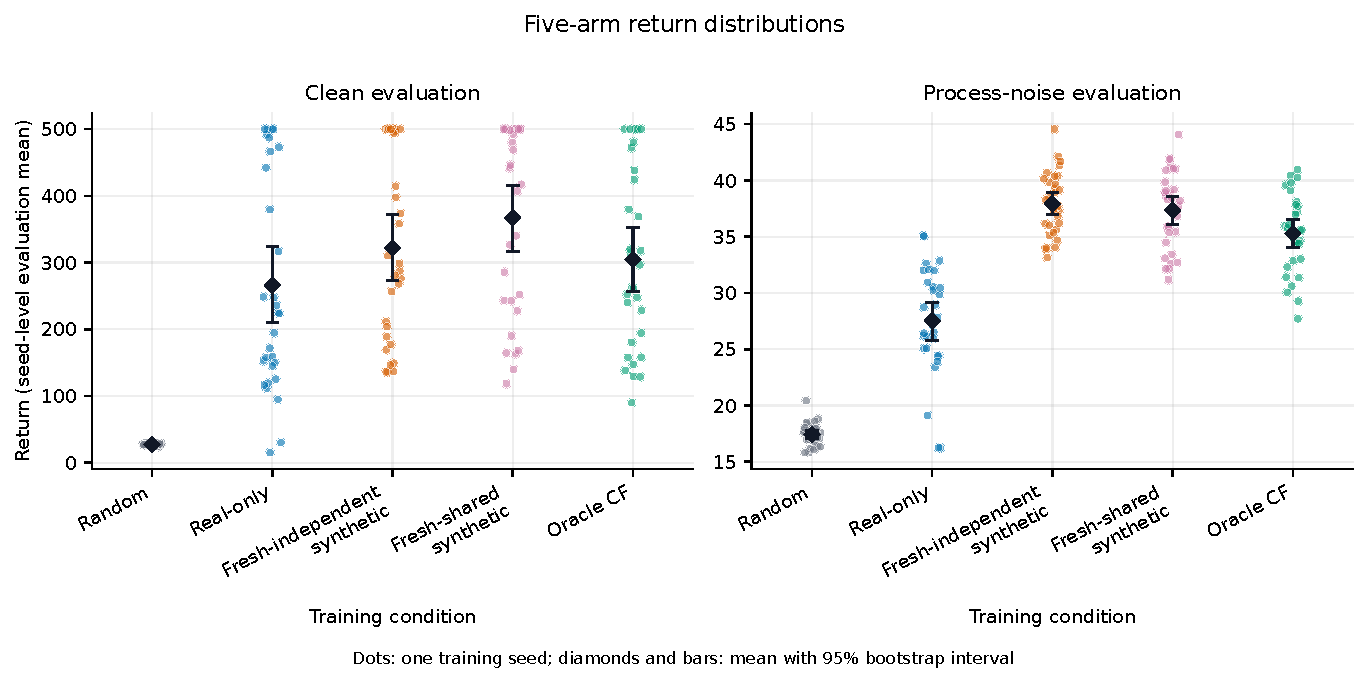
\includegraphics[width=\linewidth]{five_arm_seed_distributions_clean_process_noise.pdf}
\caption{Seed-level returns for the matched follow-up. Points are training-seed
means; diamonds and bars show mean and 95\% bootstrap interval. The evaluation scales
are separated.}
\label{fig:arms}
\end{figure}

The primary oracle-minus-fresh-shared clean difference is $-62.78$ (95\%
paired bootstrap interval $[-111.31,-14.56]$). Oracle is lower in 20 seeds,
higher in 5, and tied in 5; the paired median is $-47.63$. Raw $t$, Wilcoxon,
and randomization $p$-values are .0193, .0080, and .0192. After Holm adjustment,
they are .0580, .0241, and .0575. Thus, the direction is consistent, but
familywise significance is test-dependent, and the interval does not establish
that harm exceeds the study-defined 25-point operational threshold.

Under process noise, oracle is 2.05 points lower than fresh-shared (95\%
bootstrap interval $[-2.93,-1.13]$) and its 90\% interval lies within
$[-5,5]$. It therefore meets our study-defined practical-equivalence rule while
remaining statistically lower. Fresh-shared minus fresh-independent is
inconclusive on clean evaluation ($44.88$, 95\% interval
$[-16.46,103.68]$) and also meets the $\pm5$ rule under process noise
($-0.60$, 95\% interval $[-1.49,0.31]$).

Figure~\ref{fig:deltas} displays every seed-level primary difference and makes
the sign imbalance, ties, and wide effect distribution visible.

\begin{figure}[H]
\centering
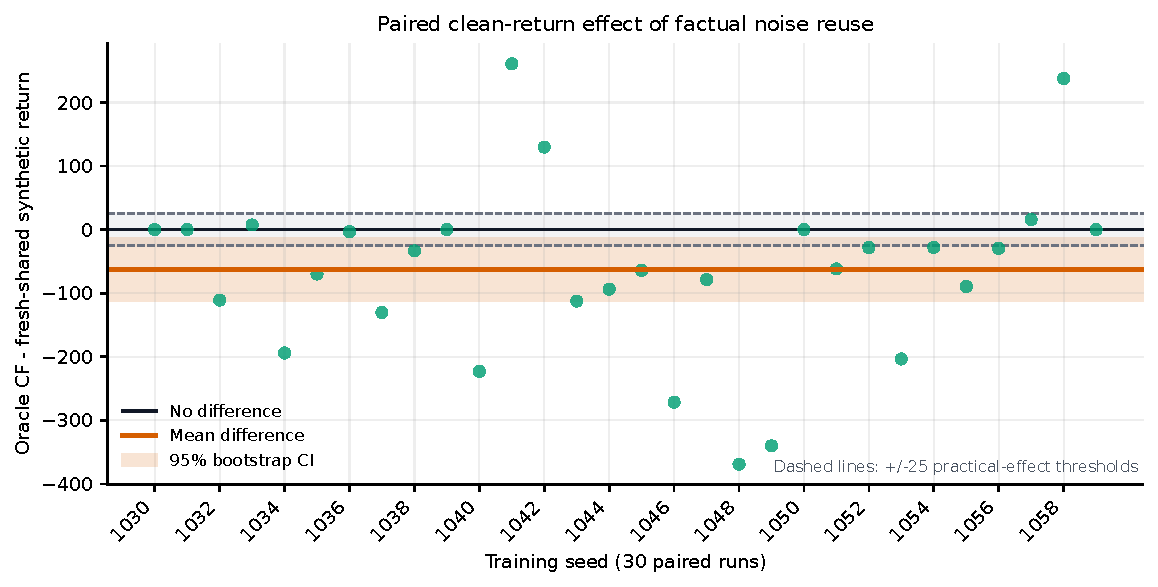
\includegraphics[width=\linewidth]{oracle_minus_fresh_shared_clean_deltas.pdf}
\caption{Paired oracle-minus-fresh-shared clean-return differences. The solid
line and band show the mean and 95\% paired bootstrap interval; dashed lines
mark the study-defined $\pm25$ practical thresholds.}
\label{fig:deltas}
\end{figure}

\subsection{The learned SCM fails its gate}

The learned-CF normalized MSE is 21.4--29.5 times the fresh-noise-to-oracle MSE
across five development seeds. Terminal disagreement is 42.0--65.9\%, every
seed has at least one latent dimension outside its accepted range, and action
reconstruction passes in only three seeds. The supplementary archive includes
the per-seed transition-fidelity and termination-consistency diagnostic. No
learned-CF policy is therefore reported.

\begin{table}[H]
\centering
\caption{Held-out BiCoGAN development gates. Eligibility required every gate in
every seed; normalized MSE is relative to state scale.}
\label{tab:model-gates}
\small
\begin{tabular}{@{}p{0.34\linewidth}p{0.22\linewidth}p{0.23\linewidth}r@{}}
\toprule
Metric & Gate & Observed across seeds & Passed \\
\midrule
Learned/fresh normalized MSE & $<0.8$ & $21.4$--$29.5$ & 0/5 \\
Terminal disagreement & $<0.05$ & $0.420$--$0.659$ & 0/5 \\
Latent SD, each dimension & $[0.5,2.0]$ & at least one violation/seed & 0/5 \\
Action/baseline MSE & $<0.9$ & $0.863$--$0.931$ & 3/5 \\
\bottomrule
\end{tabular}
\end{table}

Table~\ref{tab:model-gates} makes the aggregate decision explicit: three gates
fail in every seed, while action reconstruction alone passes in three seeds.

\section{Discussion and Limitations}

The matched follow-up rules out one explanation for the initial result: fresh
augmentation did not win solely because it used ten independent sibling noise
draws. Even after matching sharing, factual-noise reuse has lower clean mean
return. This supports a narrow conclusion: exact counterfactual coupling is not
sufficient to outperform fresh-shared augmentation for this learner, dataset,
and mixing rule. It does
not imply that counterfactual augmentation is generally harmful. Both synthetic
controls use the true simulator, whereas practical CTRL must estimate the SCM,
reward, and termination behavior.

The matched contrast is still an operational comparison, not a pure test of
causal identifiability. Reusing factual noise also couples each synthetic sibling
to the real transition present in training, whereas fresh-shared noise does not.
The effect can therefore include real--synthetic redundancy and changes in
effective sample size. Fresh-shared and fresh-independent also begin from the
same random-number stream but consume it differently, leaving one identical
synthetic next state per seed (about 0.003\% of either pool). This negligible
overlap cannot explain the reported contrasts, but distinct stream offsets
would be preferable in a future rerun. In the follow-up cohort, the unregistered oracle-minus-
fresh-independent clean difference was only $-17.90$ and was inconclusive; we do
not describe the follow-up as a replication of the initial effect.

Several limitations remain. First, the original paper's failure, convergence,
mixing, and evaluation details are unavailable, preventing exact attribution of
the reproduction gap. Second, CQL and the compact network make the mechanism
study intentionally different from CTRL. Third, clean returns are ceiling-heavy
and variable, motivating paired results and sensitivity tests. Fourth, our
positive-weight generator is nondecreasing rather than proven strictly
monotone, and its empirical failure cannot adjudicate the CTRL theorem or
BiCoGAN generally. Finally, this revision removes prior LunarLander, MuJoCo,
SAC, and D4RL rows: they were underpowered, lacked a valid continuous-action CF
definition, or did not contain a CF condition. Broad external-validity claims
require new, compute-matched studies after the learned SCM passes task-specific
state, reward, and termination gates.

\section{Conclusion}

Our audit does not reproduce learned CTRL. It shows why environment
learnability, exact counterfactual coupling, and learned-model validity must be
tested separately. A stabilized learner reaches nontrivial CartPole performance,
but exact factual-noise reuse is lower than a matched fresh-shared simulator
control on clean evaluation and meets the study-defined process-noise
practical-equivalence criterion. The attempted learned SCM fails independent validation by a wide
margin. These negative results replace the earlier broad benefit claim with a
reproducible boundary: under the tested protocol, noise reuse provides no
advantage over the matched fresh-shared simulator control, and learned
augmentation should not proceed without explicit
counterfactual-quality gates.

\paragraph{Artifact availability.}
The artifact is available in the
\href{https://github.com/ksajan/ECE595-Causal-RL-Study/tree/claramas-2026-revision-v1/publication_revision}{versioned public project archive}.
It contains frozen manifests, source hashes, exact
commands, seed-level JSON artifacts, summarizers, tests, and figure scripts.
Because the remote checkout did not expose Git metadata, the archive itself is
the authoritative source snapshot.

\appendix
\renewcommand{\theHsection}{appendix.\Alph{section}}
\section{Protocol Sensitivity Details}

Table~\ref{tab:protocol} reports the full matrix behind the protocol range in
Section~4.1. The matched-noise evaluation uses the state-noise semantics named
in each row; it is not one common process-noise evaluation.

\begin{table}[H]
\centering
\caption{Development-only protocol matrix over ten seeds (mean $\pm$ SD).}
\label{tab:protocol}
\small
\begin{tabular}{@{}llrrr@{}}
\toprule
State noise & Trial rule & Transitions & Clean & Matched noise \\
\midrule
Process & Stop & 3,494 & $32.34\pm18.16$ & $18.83\pm2.41$ \\
Process & Continue & 5,000 & $34.56\pm11.07$ & $19.13\pm1.84$ \\
Observation & Stop & 4,663 & $18.35\pm5.72$ & $17.97\pm5.33$ \\
Observation & Continue & 5,000 & $21.42\pm4.08$ & $20.57\pm3.34$ \\
\bottomrule
\end{tabular}
\end{table}

``Continue'' advances the custom dynamics after the pre-noise failure boundary
to preserve 20 consecutive transitions; it is a sensitivity analysis, not a
claim about the unpublished original implementation. Process versus observation
noise under continuation changes clean return by 13.14 points (95\% paired
$t$ interval $[6.62,19.66]$), but neither interpretation approaches the
original plot with the reported-architecture learner.

\section{Initial Oracle Study}

Table~\ref{tab:initial-arms} gives the marginal arm summaries from the first
30-seed exact-simulator study. Its oracle-versus-fresh-independent comparison
motivated the matched follow-up, but the design changed both factual coupling
and sibling-noise diversity. The cohorts are therefore reported separately and
are not pooled.

\begin{table}[H]
\centering
\caption{Initial exact-simulator study over 30 training seeds (mean $\pm$ SD).}
\label{tab:initial-arms}
\small
\begin{tabular}{@{}lrr@{}}
\toprule
Arm & Clean & Process noise \\
\midrule
Random & $26.93\pm1.58$ & $17.08\pm1.02$ \\
Real only & $272.90\pm165.71$ & $28.21\pm5.13$ \\
Fresh-independent & $335.49\pm122.94$ & $38.61\pm2.94$ \\
Oracle CF & $280.08\pm119.55$ & $36.73\pm3.92$ \\
\bottomrule
\end{tabular}
\end{table}

Oracle minus fresh-independent clean return was $-55.40$ (95\% paired
bootstrap interval $[-98.94,-9.54]$), with 21 negative, 7 positive, and 2 tied
seed differences. In the later follow-up cohort, the analogous unregistered
oracle-minus-fresh-independent difference was only $-17.90$ and inconclusive.
This heterogeneity reinforces why the fresh-shared comparison, rather than a
pooled post-hoc estimate, is the primary mechanism result.

\section{Artifact Integrity and Model Diagnostics}

The follow-up contains every seed from 1030 through 1059 exactly once. Every
artifact records the same manifest hash (prefix \texttt{0dbb740b}), source
digest (prefix \texttt{b9b2c137}), combined source/manifest digest (prefix
\texttt{d140ab2b}), configuration, and software environment. Factual
state, action, reward, next-state, terminal, and trial-index arrays are asserted
identical before constructing the three synthetic pools. For fresh-shared and
oracle CF, the maximum within-transition action- and state-noise reuse error is
zero in every run. Each synthetic pool contains exactly ten transitions per
factual transition.

The archive includes all raw JSON files and validators. From a clean
environment, 50 focused tests pass; the four principal summaries regenerate
byte-for-byte; and both PDF and PNG figures regenerate from the stored
summaries. Git metadata was unavailable on the remote execution checkout, so
the exact archived files and their hashes, rather than a remote commit field,
bind code to results.

Figure~\ref{fig:modelgate} shows the two largest learned-model failures. The
transition ratio is more than 21 rather than below 0.8, and terminal
disagreement is at least 0.42 rather than below 0.05. These are development
diagnostics, not downstream confirmatory evidence.

\begin{figure}[H]
\centering
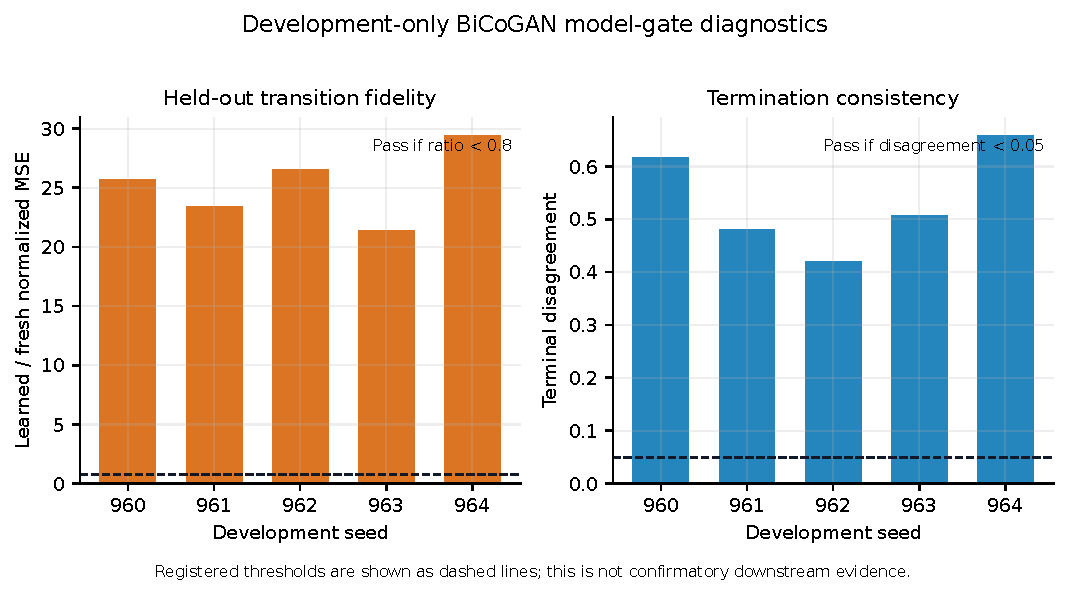
\includegraphics[width=0.92\linewidth]{model_gate_fidelity_and_terminal_disagreement.pdf}
\caption{Held-out development diagnostics for the attempted BiCoGAN. Dashed
lines are manifest-specified gates, not fitted decision thresholds. Both shown
metrics fail every seed.}
\label{fig:modelgate}
\end{figure}

\bibliographystyle{splncs04}
\bibliography{references}

\end{document}
